\documentclass[letterpaper,10pt]{article}
\usepackage[utf8]{inputenc}
\usepackage{authblk}
\usepackage[margin=2cm]{geometry}
\renewcommand{\baselinestretch}{1.5}
\usepackage[round]{natbib}
\usepackage{hyperref}
\usepackage{graphicx}
\usepackage{caption}
\usepackage{subcaption}


%Getting the paper ready for journal
%Modifications due to reviewers comments


%opening
\title{Population as Auditor of an Election Process in Honduras: VotoSocial}
\author[1,2]{Carlos Roberto Arias (cariasa@unitec.edu)}
\author[1,3]{Jorge Antonio Garcia (jorge@icoms.co)}
\author[3]{Alejandro Corpeño (corp@icoms.co)}


\affil[1]{Facultad de Ingenier\'{i}a, UNITEC, Tegucigalpa, Honduras}
\affil[2]{Instituto de Investigaci\'{o}n de Pol\'{i}ticas P\'{u}blicas, UNITEC, Tegucigalpa, Honduras}
\affil[3]{Icoms Technologies S de RL, Tegucigalpa, Honduras}

\begin{document}

\maketitle

\begin{abstract}
For a country to become fully democratic the majority of the population needs to be involved in the politics of the country. Involvement requires people to be aware of what is happening, and to be able to participate in the political processes of the country. Crowdsourcing systems penetrate the social media, and by doing so they allow the general population to actively participate in the political life of their country. VotoSocial is a crowdsourcing system that was born during the 2013 government elections in Honduras, it was used to retrieve the official digital records of the government elections authority: The Supreme Electoral Tribunal, and then providing them to the internet community to digitise these records and to verify their digitisation. VotoSocial was able to verify the accuracy of the official results as they were given by the Supreme Electoral Tribunal. It was found that there was no fraud in the digitisation process, but further statistical analysis showed a data behaviour that is usually seen when there is incremental fraud in an electoral process. VotoSocial as a system has proven that social media powered crowdsourcing systems can provide the population with political awareness in a government elections, thus opening a clear opportunity to build more platforms as this one.
\end{abstract}

\section{Introduction}
It is accepted among Hondurans that the government is corrupt, this is supported by the evidence found by Transparency International that rates Honduras with a score of 26, with only 37 other countries considered to be more corrupt than Honduras \citep{transp}. This fact is affecting the Honduran society in many dimensions, one of them is the impact it has on the education and thus the democratic maturity of the general population. With a 14.5\% of the population above 15 years of age that cannot read or write \citep{bchrep}, and with 64.5\% of the population living under the line of poverty \citep{wbdata}, this country's educated people is a minority.


However a minority can have a powerful impact in the country, when even a small group can shake the status quo of a government \citep{saadia2014} as it has happened in the recent government elections held in October 2013. During this process a crowdsourcing system was built called VotoSocial: \url{http://votosocial.org}, where 97\% of the presidential polling records where reviewed by the people participating with the system.

In this electoral process eight political parties participated for the president position, one of the candidates being the former President of Congress. This fact and the previous turmoil produced by the events of 2009 where former President Manuel “Mel” Zelaya was deposed, had the country in a state of tension. Even with the political stress, this past elections proved to be representative as more than 60\% of the registered voters participated with their votes. In addition to the high turnout, in this elections the official polling tables records were digitalised and made public by the Supreme Elections Tribunal (TSE) through their elections site SIEDE: \url{http://siede.tse.hn}. In Honduras the elections are organised as follows: the country has departments, each department has municipalities, each municipality has voting centers, and each voting center has polling tables. Voting centers are places that are located near the population to enable domiciliary voting, and to make the process more efficient in each voting center several polling tables serve as places where the citizens actually put their vote.

During the process there was a perception that the elections were fraudulent, specifically the process of digital input of the records to the TSE computer system. Most of this perception was due to the political power that one of the candidates had at the moment of the elections, as pictures of inconsistent polling records favouring this candidate appeared in social media, and partly because of the awareness of the general public of the corruption of the government. The lack of confidence in the elections system of Honduras can be seen in the infamous statement by former president Zelaya where he stated that it is necessary to have a 10\% fraud to be able to beat the system \citep{melvid}, additionally studies have shown that only 23\% of Hondurans believe in the electoral process \citep{romero2014}.

Considering all these facts, some people started to organise procedures to check the official records, and to find a way to report this to the general public. Some used Facebook as their propagation method, and Google Docs as a way to register the potential anomalies found in the counting process of the official polling records. Some other people, among the authors of this paper, decided to take this a step further, and developed the \textit{VotoSocial} platform, to allow people to verify the government counting of the official polling records.

Democracy is not an easy feat, especially in a developing country as Honduras, but crowdsourcing systems like \textit{VotoSocial}, can help a minority of a population have a deep impact in the society, allowing some of the more educated people help discover anomalies in the government proceedings, making this information public and explaining how this affects the general public. Furthermore, this initiative allowed users that would just complain about the government in Facebook, to use their energy in a positive constructive way, and to involve them in the political life of their country, something that they would not have been able to do without \textit{VotoSocial}.

These kinds of systems will help society get a better participation in the governance of a country, because they will make people be heard by their government and will increase general public awareness. In addition to these benefits, \textit{VotoSocial} provides a path to a more transparent electoral process, so much that it has serve as an inspiration to other crowdsourcing systems like the one developed by \citep{contemosnosotros} in the neighbour country of El Salvador. 

Following this introduction a brief background description of crowdsourcing and the political history of Honduras is presented, after this a panoramic view of the elections in 2013 is shown, followed by a statistical analysis that the \textit{VotoSocial} platform allowed to do. Finally future and potential work is described and conclusions are given.


\section{Background}

\subsection{Crowdsourcing}

Cyberactivism is reshaping the way that policy has traditionally been conducted, whose perspectives are included and how awareness is risen among the people \citep{milan2013}, cyberactivism activities include among others crowdsourcing. Crowdsourcing is a process where an online community collaborates to reach a goal, where each participant contributes with a small portion, and these contributions are later integrated to provide a solution to a bigger problem. In a manner, it builds a big solving machine using humans as computational components, thus enlisting people to solve a variety of problems \citep{doan2011}.

According to \cite{doan2011} crowdsourcing operations need to consider the amount of manual effort, the role of the human users and whether the system is going to be standalone or piggy-back on another system. The amount of manual effort refers to how much time and effort each human user is expected to give to the system, most systems expect very little from users, and work with a considerable number of users. Additionally, the function of these users needs to be clearly established, in such a way that it is difficult for users to introduce noise to the solution of the problem at hand. Lastly, some systems rely on the existence of another system, creating a symbiotic relationship, for instance the reCAPTCHA (\url{https://www.google.com/recaptcha/intro/index.html}) system that piggy-backs on other systems to help digitise text, annotate images and help in the building of machine learning datasets; some other systems are standalone such like the SETI@Home (\url{http://setiathome.berkeley.edu/}). In addition to these considerations, there are several dimensions of crowdsourcing that establish how to recruit and retain the users, what each user can do, how to combine their contributions and how to evaluate them. For instance in one crowdsourcing solution for disaster relief \citep{gao2011}, users would be recruited by letting a wide range of the population know the availability of the system, in this instance people use Twitter to send information messages. The retention of users is achieved by the good will of people to collaborate with the emergency relief efforts. Users only needed to send their tweets with a identifiable hash tag and location, and then the system would combine these tweets by mining the tweets. This particular system had the challenge of data validation, but it serves as a good example on how these dimensions need to be dealt with.

Crowdsourcing systems do not exist without problems and challenges, among them there is the need to evaluate the correctness and validity of the user contributions, how to reach enough users to have a significant contribution to the system and how to make people accountable for their participation. Each crowdsourcing system faces these challenges their own way, depending on their specific goals and domain.

Needless to say that thanks to social media, crowdsourcing offers a powerful tool to collect information and users can also be used to validate the data \citep{gao2011}. Successful stories on how crowdsourcing has been used can be found around the globe, like its usage in disaster relief \citep{yin2012, gao2011} and its use in the electoral process of Honduras and El Salvador in 2013.

For crowdsourcing systems to be successful they need to keep its human users motivated, this can be achieved by convincing them of the necessity of the service, instant gratification, fame and reputation \citep{doan2011}. The last two factors can be reached by attaching a social media component to the crowdsourcing system, so that users can show off their accomplishments with their peers. The use of social media also helps with the challenge of reaching more users, in addition to become a source of information and communication \citep{yin2012}, and helps political bodies as a mean to gather support, mobilise people and to get political messages spread \citep{map2014}.

By involving social media, many of the crowdsourcing challenges are faced and solved, and in addition the systems get a broader audience, so that results can also be shared with more people, providing better situation awareness, new paths of communication and opportunities for assistance \citep{gao2011}. However the crowdsourcing systems need to provide appropriate and rapid response and results to keep active and collaborating users, and passive and read-only users engaged with the system.


\subsection{Honduras Political History}

Honduras political history is marked with bipartisanism between the Liberal Party and the National Party, and the frequent military government in between. The longest, and most remembered, dictatorship was by General Tiburcio Carías in 1932, and when it finished in 1948 the country started its tendency to democracy.

Following the dictatorship that lasted from 1932 to 1948, the General Tiburcio Carias called for elections. However the results of this process were already arranged in such way that Juan Manuel Gálvez, from the National Party, won this elections with 99.8\% of the votes in favor. Later, in 1954 presidential elections were held again, the opposition party, the Liberal Party won the elections, but since the law required an absolute majority, the Vice President took over the government. In 1956 the opposition of the ruling government was persecuted, a candidate was exiled and state resources were mobilised to enable clientelism: the exchange of services or goods for political favour. By means of fraud the government party achieved 89.4\% of the votes and full representation in Congress \citep{romero2014}. This election was followed by a coup d'\'{e}tat, and after that a Constituent Assembly was brought, later called for elections where Ramon Villeda Morales, a Liberal Party militant, was elected President, he was later deposed by another coup from the military. This military government called again to elections, and the elected President Ramon Ernesto Cruz, was also deposed by the military a little more than a year later of being elected. During the military government a new Constituent Assembly was called, a new Constitution was written, and elections were called again in 1982.

From 1948 to 1980 coup d'\'{e}tat, fixed elections and fraud where interleaved until in the early 1980's a new National Constitution was written and an electoral process began again in 1982. Democracy was then restored, and has continued periodically every four years, without interruption of the military raising to power. The only exception to this democratic continuity was the deposition of President Manuel Zelaya, from the Liberal Party, in 2009. A factor affecting the political turmoil from 1948 to 1980 was that the scarce available media was unable to work well due to the restrictions of freedom of speech, along with low education levels that yielded very low situation awareness.

During this democratic streak, fraud has not been as crude as it was 30 years ago, and Honduras has been in the vanguard of electoral process in comparison to its immediate neighbours, for instance the advances in 1997: established one ballot, domiciliary voting, use of national ID card as voter registration \citep{romero2014}.

The events around the 2009 political crisis, when elected President Manuel Zelaya was deposed by Congress, and exiled by the Military, confirmed the fragile capacity of public action of Honduran society \citep{romero2014}. The following 2009 elections in Honduras had one of the lowest turnout in recent history having the following distribution of votes: 17.06\% independents, 56.05\% loyal militants, 45.97\% electoral participation, 18.47\% victory margin. According to \cite{gonza2014} during the 2009 elections 22\% of the voters participated in one form or another of vote buying. Vote buying strategy was mostly oriented to loyal militants, in the form of targeted turnout and mobilisation \citep{gonza2014}. Porfirio Lobo won this elections ending the pattern from 1982 of two liberal party governments preceding a national party government.

Survey results show that even though there is a periodicity to the democratic process, the public still does not trust the general process and transparency of the elections \citep{romero2014}, other research shows that 48.3\% believe that democracy is worst now and only 5\% is satisfied with the current democracy \citep{latinbar}. Even though Honduras is improving technically in its electoral process, there is a clear lack of confidence in the results, this is mostly due to the historical tendency to fraud and vote buying.

Elections were held in November 2013, eight political parties participated with a total turnout of 61.16\%, a significant increase from the previous elections. This elections were historically unique since they ended the usual bipartisanism that is usual around the world, in this elections the Liberal Party, one of the traditionally more powerful parties, only won in one department of the republic. Another particularity of this elections was that new political parties won whole departments, something that never happened before with any of the other smaller parties. A new party called PAC won one department, four departments were taken by LIBRE a new party derived from the Liberal Party after the crisis of 2009, and the rest of the country was won by the National Party.

The PAC party presented for the first time a different proposal, filling a vacuum that traditional parties have not been able to fill. People are expecting a top-down approach where politicians use more social media, reach the population and listen to the people using this technology \citep{map2014}. This was reflected in the elections counts where PAC achieved good results in urban areas where there is greater development, the downside was that there was little or no influence in the rural areas. An additional consequence to the usage of social media, is that this particular party attracted younger sectors that usually did not participate in the political processes \citep{romero2014}.

The National Party, represented by Juan Orlando Hernández at that time President of National Congress, mostly won in the western and southern parts of the country, in these regions there is a greater rural population, a population with less development that wanted to preserve the ``Bono 10,000'' program. During the 2010 - 14 term of President Porfirio Lobo, the``Bono 10,000'' program was created. ``Bono 10,000'' is a government program with the goal of transferring money to homes categorised as in a state of extreme poverty, with children properly enrolled in the public school system and that regularly assist to school. It is part of the Millennium Development Goals \citep{mdg2006} to eradicate extreme poverty. To reach this goal the ``Bono 10,000'' program was created as a Presidential Program for Health, Education and Nutrition \citep{bono10k}. This shows consistency with the social policy in Latin America that is characterised by ``conditioned subsidies'' \citep{romero2014}. This program started by former President Porfirio Lobo is continued by current President Juan Orlando Hern\'{a}ndez. 

During the 2013 elections middle and upper class had higher turnout rates, urban lower class contrasted with rural people that are more participative, political parties networks worked very well in rural parts of the country \citep{romero2014}. This behaviour as expected shows how low income citizens usually respond positively to immediate benefit \citep{kit2000}, according to the study done by \cite{gonza2014} is a conduct seen in developing countries, which relates to the correlation between gross domestic product and vote buying . Evidence corroborates that social benefits for lower income classes, makes these people more susceptible to vote buying, thus showing that the rational theories are held in Honduras \citep{gonza2014}. Besides income, the other factor affecting the vote is the intensity of political sympathy, that may result in the mobilisation of followers. This form of vote buying takes the shape of electoral participation buying. This is consistent to the voters behaviour in the United States where socioeconomic status correlates to geographical location of voters and also to political preferences of voters \citep{osborn2010}.

Another characteristic of the 2013 elections was the participation of eight political parties. Having so many political parties opened the door to polling tables credentials traffic, a form of electoral fraud where people from one political party hold a credential of representing a person from a different political party, thus increasing the control in the polling tables. This was seen during the 2013 elections and documented in a TV interview where a representative of the National Party was holding a credential of another Party \citep{vidap}. The polling table remains the weak link in the electoral process as this is the least supervised spot \citep{romero2014}. Bigger and traditional parties usually possess resources and have a greater capacity to turn on the vote buying machinery. To achieve this, it requires knowledge of the local population, budget, trust networks, judicial protection \citep{gonza2014}. Judicial protection was achieved by current president, at the time that he was president of Congress by dismissing four Supreme Court Justices, specifically the ones in charge of declaring violations to the National Constitution \citep{csj2012}.


\section{Government Elections 2013: The Birth of VotoSocial}

In the midst of the official vote counting by the Supreme Electoral Tribunal (TSE), VotoSocial is born. As it was discussed earlier, there was an atmosphere of distrust towards the vote counting, this contributed to the creation of VotoSocial. VotoSocial is a crowdsourcing platform that allows users to verify scanned digital polling table records, and to transcribe the values into a computational system. Figure \ref{fig:main} shows a screenshot of VotoSocial main page.

\begin{figure}[h!]
    \centering
    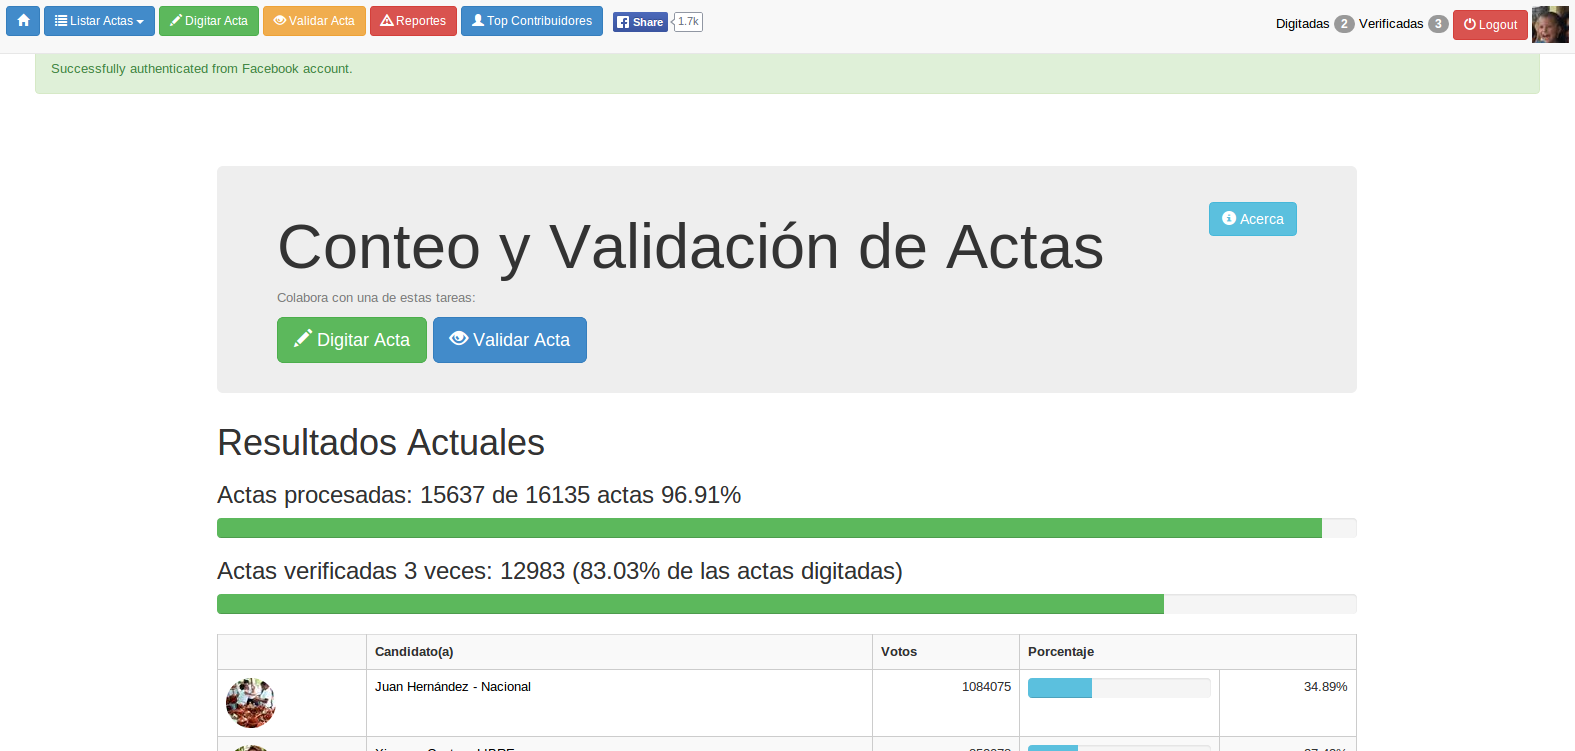
\includegraphics[width=0.8\textwidth]{images/vs-main}
    \caption{VotoSocial Main Page}
    \label{fig:main}
\end{figure}


VotoSocial team grabbed all the digitalised polling records. The process of retrieving these records was done in batch, downloading the records as these were being made available by the TSE. VotoSocial then allowed the system's users to see the scanned record, and to register the values, digitalising this way the results of each of 15,637 polling tables, this represents almost 97\% of all the polling stations in the country, the remaining 3\% was not verified as these records were never made public by the TSE. Users were also in charge of the validation of this process, so every time a transcription user digitised a record, three different users had to validate that this transcription was correct. There were 6,232 unique visits to the site, 1,673 people registered in VotoSocial, 710 users were actively transcribing records, and 879 people participated reviewing the transcriptions. The whole process took six days, however it was done altogether in less than 48 hours. In the first day programming and testing was done and 1\% of the records were processed, during the following two days 88\% of the records were processed, hours after these were available for the VotoSocial users. The rest of the records were processed during few hours in the last three days.

According to \cite{doan2011} VotoSocial architecture is explicit and assigns the users with task execution, all effort is done online, and unlike other systems that send tickets when a user finds a mistranscription \citep{haaf2013}, the correction is done online and almost in real time. Still, users may send reports when they found suspicious records like the one that can be seen in Figure \ref{fig:strange}. In an effort to find correct results a method of triple verification was used, this allowed for a user controlled validation of the data. For a record transcription to be accepted three different persons had to review and check that the record has been correctly transcribed. The motivation behind triple validation was to have a system like the double keying systems \citep{haaf2013}, but it was decided that triple validation would be more user friendly and would provide a better user experience, without loosing accuracy, and enabling the community to automatically validate the digitisation process. The system becomes more user friendly, and with a better user experience than double keying systems as it only requires a single click on a button to acknowledge that a transcription is correct or incorrect, thus making the system easier to use, and allowing faster processing; in double keying systems all users need to input the whole amount of text that is being digitised. See Figure \ref{fig:strange} that on the bottom left has two buttons to recognize the transcription to be correct or incorrect.

A better system was implemented by ``Contemos Nosotros'' \citep{contemosnosotros} system made in El Salvador following the example of VotoSocial, in this system the user does not know what party he is digitising the values for, as shown in Figure \ref{fig:salvador}, the user only sees the digital picture of the numbers, this allows for a more transparent system of digitisation, but unlike ``Contemos Nosotros'' VotoSocial needs the user to login using a Facebook or Google+ account thus providing a level of accountability from the users. Users were recruited using social networks as Facebook and Google+, basically taking advantage of the word of mouth (By liking the page on their Facebook or Google+). Data was integrated by simple addition, so integration was not actually a challenge of the platform. Opposed to other crowdsourcing systems, VotoSocial did not form a community as such, since there was not explicit communication between the users inside the platform. Decisions were always made agilely by the system operators taking user comments into account, much the way a software is developed nowadays. The operations that users were allowed to do were as digitisers and reviewers. Digitising consisted in transcribing the official record, and reviewing consisted in the revision of this transcription. Another difference between VotoSocial and other crowdsourcing systems and to cyberactivism sites is that VotoSocial was not anonymous, this was decided to encourage accountability of the users and their actions inside the system. 

\begin{figure}[h!]
    \centering
    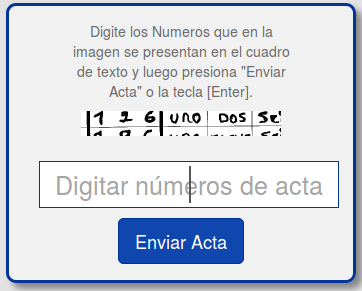
\includegraphics[width=0.2\textwidth]{images/salvador}
    \caption{ContemosNosotros Platform Partial Digital Record Digitisation}
    \label{fig:salvador}
\end{figure}


Some of the shortfalls of other crowdsourcing systems, like the one presented by \cite{gao2011}, is that it is difficult to coordinate the collaboration between all the users of the system, sometimes the provided information by the users is not verified or inaccurate, and another issue is the security of the people involved. None of this shortfalls were encountered by VotoSocial, coordination and verification was automatic by the triple verification scheme, and the security of the users was not compromised as this system was never seen as a threat to the government or its institutions.

\begin{figure}[h!]
    \centering
    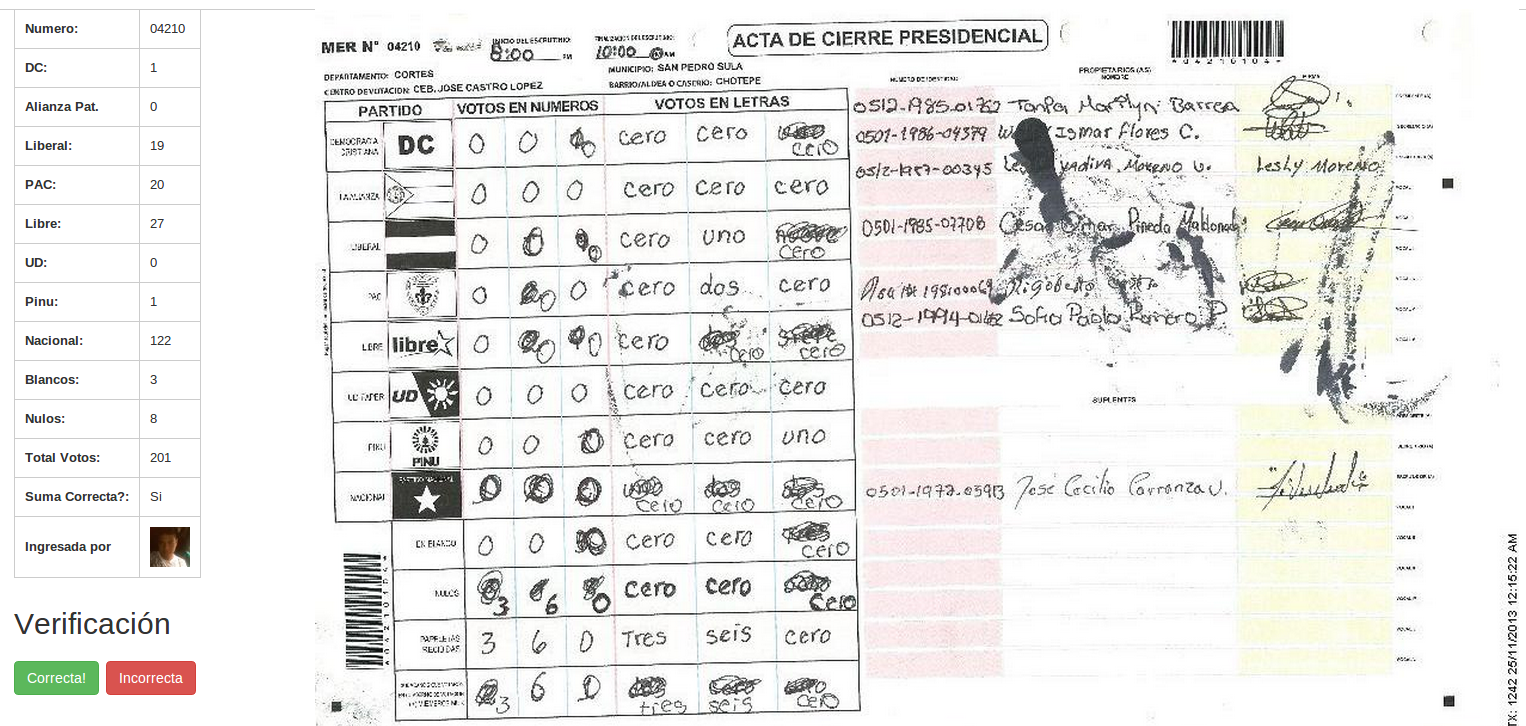
\includegraphics[width=0.8\textwidth]{images/vs-valid-strange}
    \caption{Suspicious Polling Table Digital Record Inside VotoSocial Platform, on the lower left can be seen the buttons to verify that the record has been correctly digitised (green button) or incorrectly digitised (red button)}
    \label{fig:strange}
\end{figure}





\section{Analysis}

To be able to compare with final official results, in May 21st 2014 the authors requested official detailed data to the Public Information Access Institute \url{http://www.iaip.gob.hn/} however after three months there was no response on their behalf. Despite the lack of response, VotoSocial did not find significant discrepancies between the overall official results of the TSE web site and its own results, thus showing that at least in the digitisation process in the TSE there were no ``foul play''. Notwithstanding this, further analysis of the data showed a correlation between the percentage of voter turnout in the polling tables and the percentage of the voters of the winning candidate, where there should be none, further analysis on this is discussed in the next section.

Although the official count data was not released through the official channels, thanks to the VotoSocial platform an independent count of the votes using the official polling records was achieved. This count allowed to do additional quantitative statistical analysis to further the qualitative findings of \cite{gonza2014}.

An initial statistical analysis using the methods proposed by \cite{klimek2012} showed that there is evidence of what they called incremental fraud, but there is no evidence of extreme fraud. \citep{klimek2012} consider incremental fraud to be when voting boxes have valid votes and additional ballots from the winning party, combining real and legal votes with votes filled on purpose to help the winning party, or by taking away votes from the other parties. On the other hand there is extreme fraud where some voting stations or districts show a 100\% turnout with 100\% count for the winning party. Figure \ref{fig:test} depict the correlation between voter turnout and votes of the winning party for three different cases. Figure \ref{fig:normal} shows how normal behaviour should look like with no smearing to either side. Figures \ref{fig:fingerprint} and \ref{fig:extreme} show a correlation with smearing to the right. For instance in Figure \ref{fig:fingerprint}, the fingerprint for the Honduras 2013 elections, can be seen a smearing to the upper right corner, an election result fingerprint associated with incremental fraud. Furthermore Figure \ref{fig:extreme} shows extreme fraud with a concentration of points in the upper right corner, showing that some voting tables had 100\% turnout and 100\% votes for the winning party. It is worthy to note that extreme fraud is not present in the data collected by VotoSocial, however the smearing clearly suggests incremental fraud took place during the Honduras 2013 government elections.

% \begin{figure}[h!]
%    \centering
%    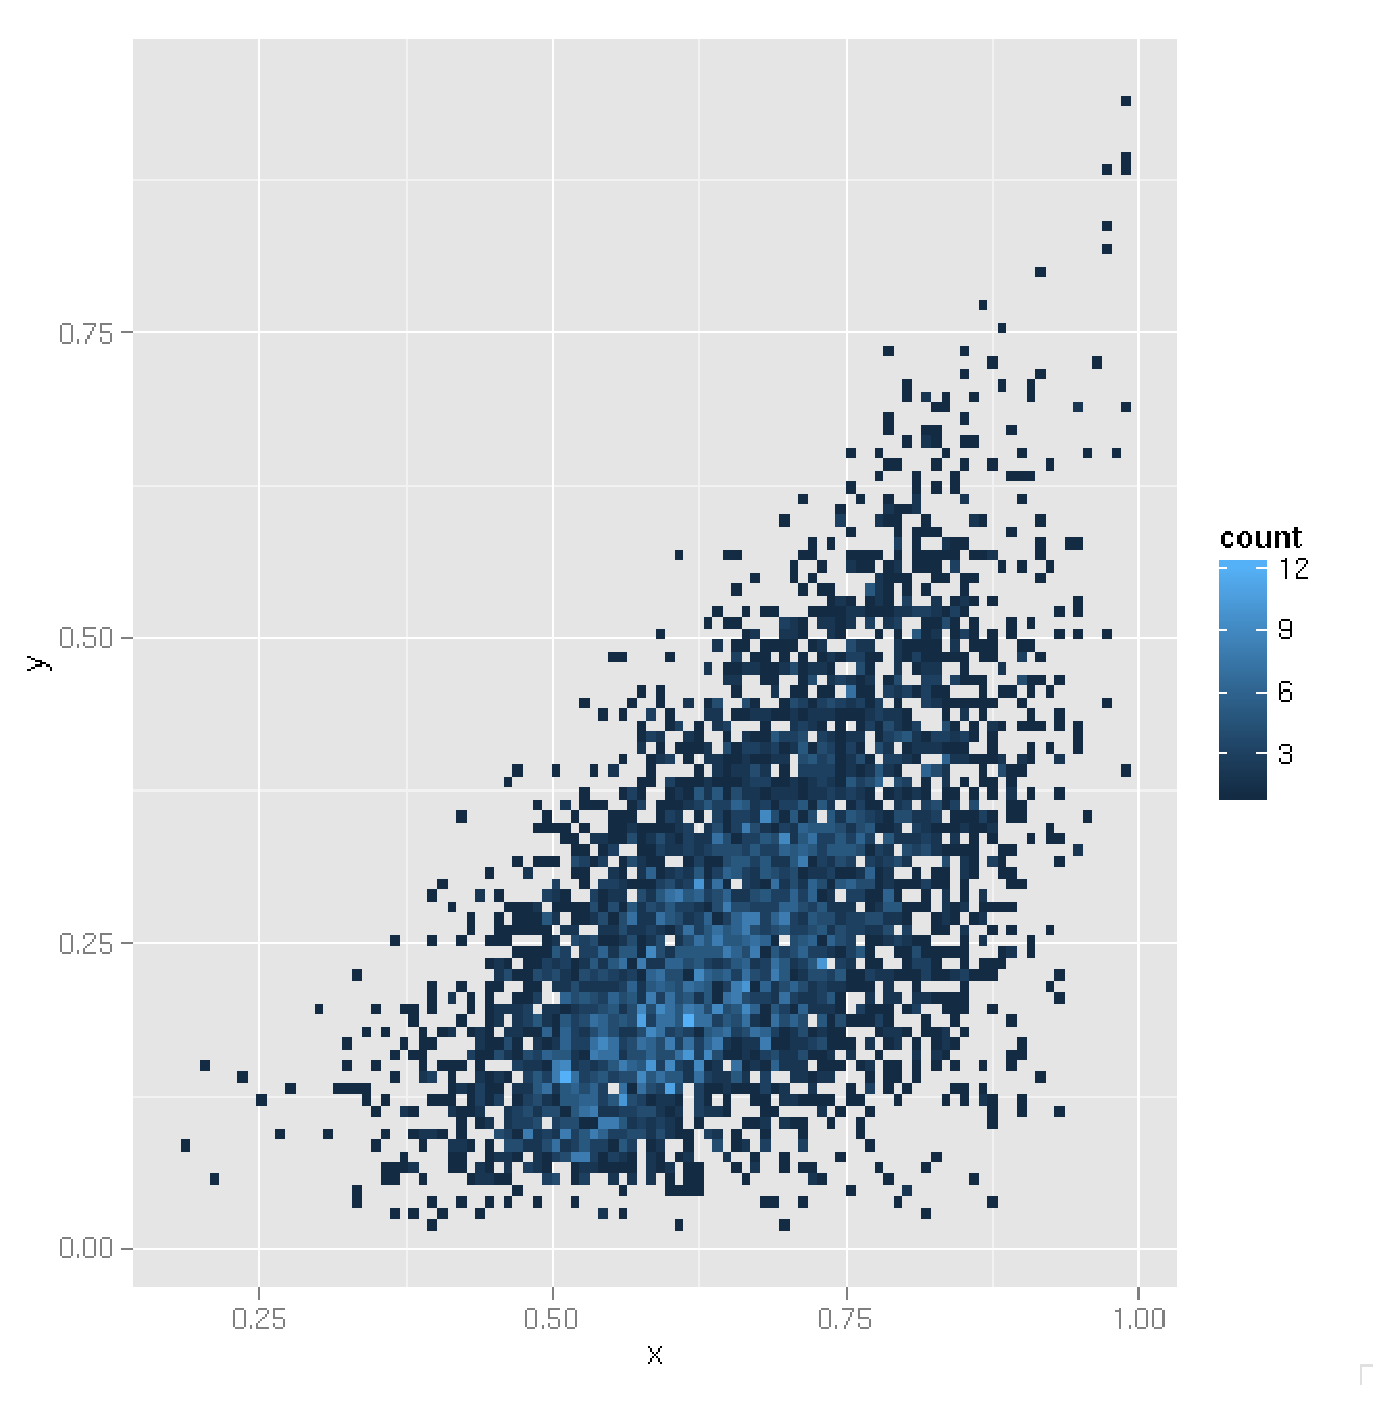
\includegraphics[width=4in]{images/fingerprint}
%    \caption{Honduras 2013 Elections Fingerprint}
%    \label{fig:fingerprint}
% \end{figure}


\begin{figure}
\centering
\begin{subfigure}{.3\textwidth}
  \centering
  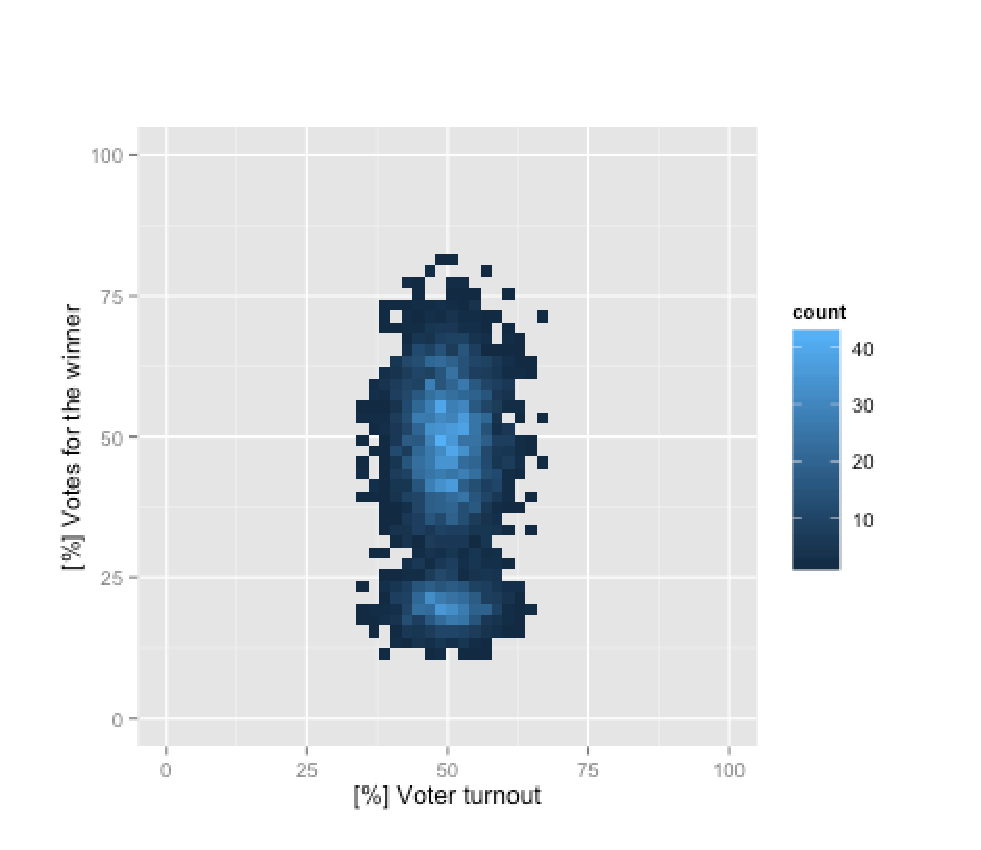
\includegraphics[width=2in]{images/normal}
  \caption{Normal}
  \label{fig:normal}
\end{subfigure}%
\begin{subfigure}{.3\textwidth}
  \centering
  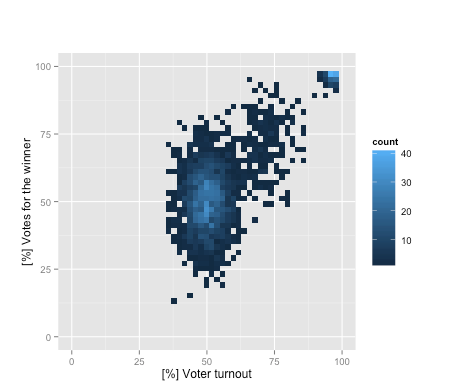
\includegraphics[width=2in]{images/extreme}
  \caption{Extreme Fraud Example}
  \label{fig:extreme}
\end{subfigure}
\begin{subfigure}{.3\textwidth}
  \centering
  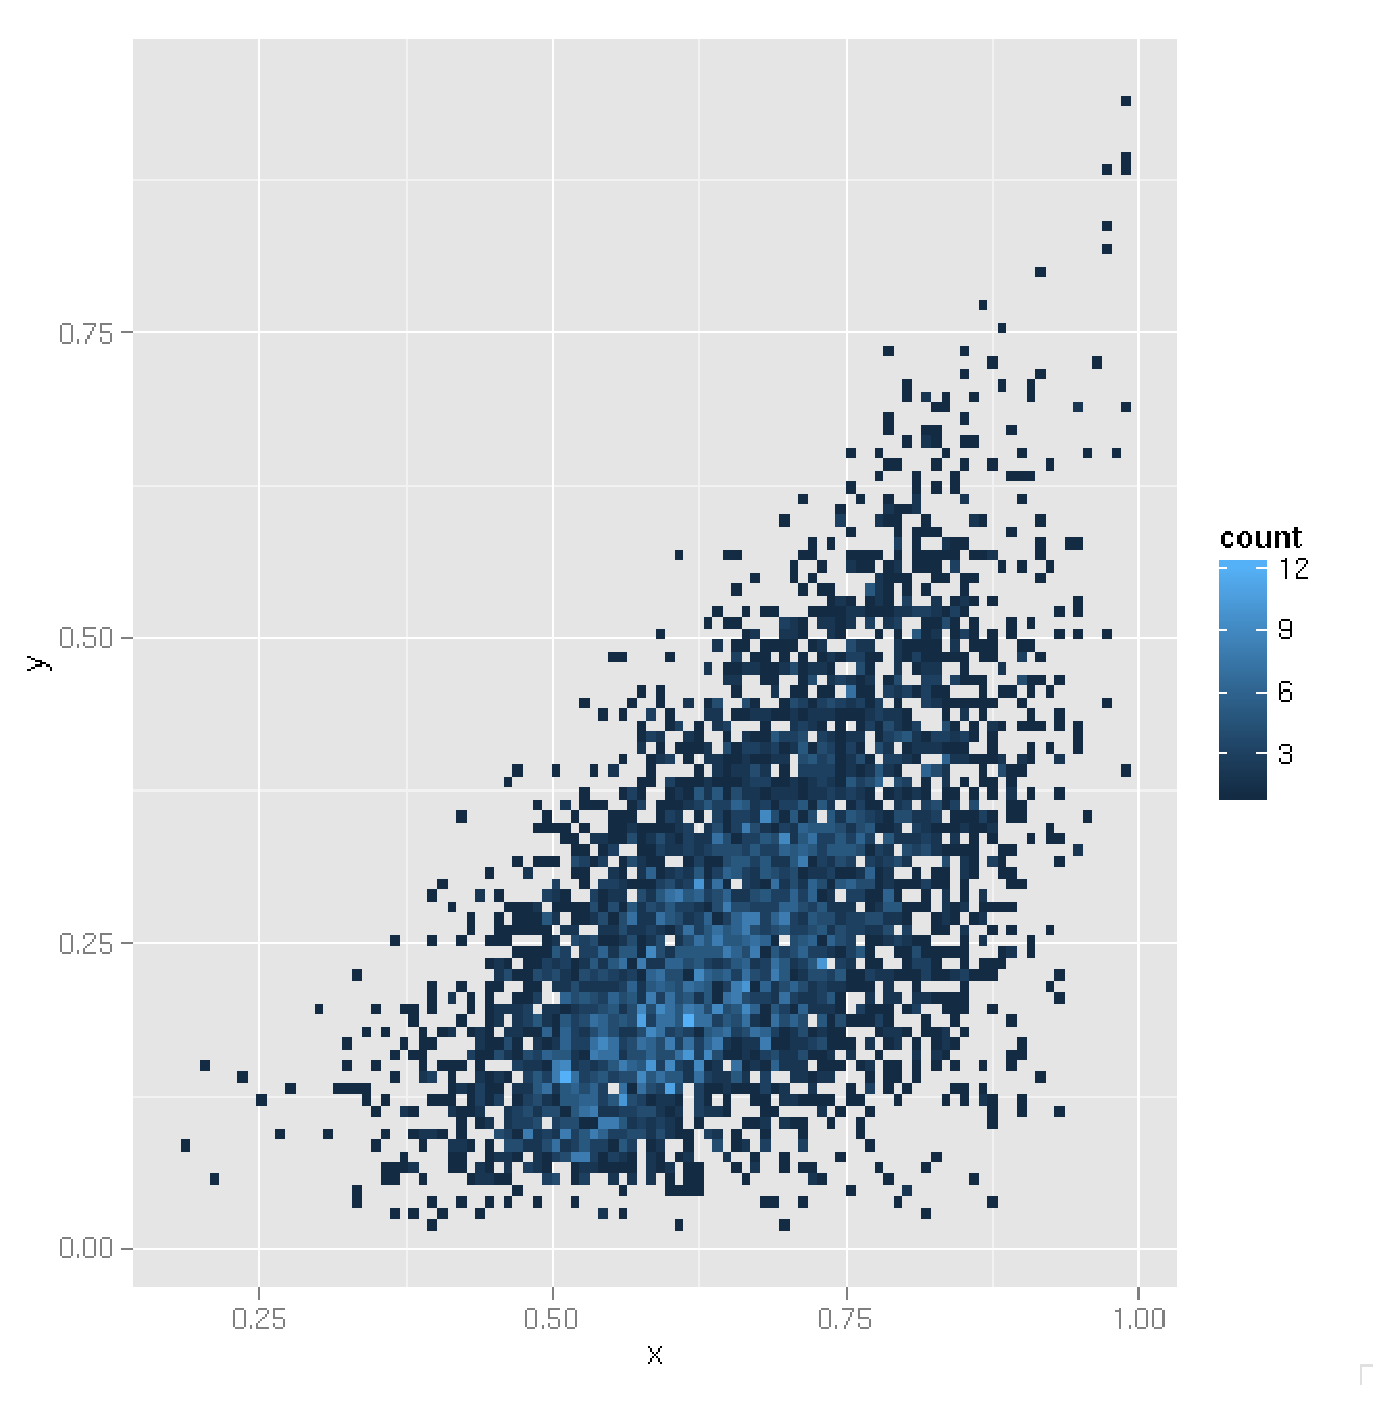
\includegraphics[width=2in]{images/fingerprint}
  \caption{Honduras Elections Fingerprint}
  \label{fig:fingerprint}
\end{subfigure}

\caption{Statistical Correlation Between Elections Turnout and Winner Votes}
\label{fig:test}
\end{figure}

In addition to the statistical findings, a survey to the participants of VotoSocial was collected. According to this survey 42.54\% of the participants expressed that they are more politically active thanks to VotoSocial, 87.31\% believe that due to the internet they can be more politically active, and 82.09\% agree that social networks have a positive influence on how politically active they are. In general, 91.04\% of the surveyed people feel that thanks to crowdsourcing platforms like VotoSocial they can be more politically active.

\section{Future and Potential Work}

\cite{doan2011} presents three major directions for crowdsourcing systems: more generic platforms, more applications and structure and more users and contributions. This proposal could be met by VotoSocial future work by: making the platform readily available for other countries election process, creating of spin-off systems for government auditing, and by increasing the Internet penetration in developing countries to reach a higher number of people from the general public.

VotoSocial started out as an open source project and its source would be available to anyone that contacts the VotoSocial team through the VotoSocial web site, or downloads the source code from the GitHub repository: \url{https://github.com/corp/ActasCounter}. In the future the software development team wishes to enable the platform for real time statistical analysis and to add more graphical reports to help the population have situation awareness about the election process as it is happening.

Additional work could be done by doing a deeper statistical analysis to check for further clues on potential fraud during an election process, such as the fraud parameters computed by \cite{klimek2012}. In addition to these indicators, an enhanced registration form would allow research on more statistical features of the participants in the VotoSocial platform, by registering demographic, socioeconomic and political data from the users.

VotoSocial may be a catalyst to the creation of spin-off for general government auditing. This crowdsourcing system would help the general public to audit and comment in a structured manner the government funded projects, in the local and national level alike. This evaluation systems could incorporate the evaluation techniques presented by \citep{morra2009}, and become an independent, people managed evaluation system, becoming the counterpart of government internal evaluation systems like the Single System of Evaluation of Social Public Policy (Sistema \'{U}nico de Evaluaci\'{o}n de Pol\'{i}ticas P\'{u}blicas: SUEPPS) \cite{arias2014}. Such systems would need to be hosted by apolitical entities such as a university or an NGO and would be fed and regulated by the community in a manner like Wikipedia, thus becoming a people managed system. Independence of such system is held by the impartiality of the supporting institution, and by the free access to citizens that would be the real auditors.

As any research and development project the major challenge is to find funding to get the necessary infrastructure and personnel to build and develop and maintain these platforms, these challenges are particularly difficult in developing countries that do not have an established research funding mechanism. Ideally personnel for software development could be enlisted the way open source projects do, however unlike developed countries, people, specially engineers, do not have as much free time to dedicate to these kind of activities.


\section{Conclusions}


In the 1948 elections there was an electoral scaffolding that far from helping a fair election used a mechanism that guaranteed the victory of the ruling party. 2013 was not much different, even with the technical advances that were supposed to boost confidence in a more transparent electoral process, the resemblance with the 1948 elections where the ruling party had electoral scaffolding and access to government resources produced a lack of confidence from the general public \citep{romero2014}.

Social media may gather people together the way Facebook and Twitter do, specially when people have a common interest. These social media platforms allow people to complain, suggest and comment, but all the information is lost in the sea of ``social text'' without structure or organisation, so it cannot be used in a meaningful way.

On the other hand crowdsourcing platforms, in addition to bringing people together and allowing people to comment and collaborate, provide structure that allows summarisation and aggregation of the data that can later be used to reach community goals. This is what VotoSocial achieved, it brought together Hondurans from all over the world to help audit the digitisation of polling 

In the world, higher turnout usually means a greater demand of the public for results \citep{mac2003}, this is not true for Honduras where abstention and comfort are not aligned, since even when there is high turnout people do not consistently demand results from the government \citep{romero2014}. Historically Hondurans have lacked the will to protest, dissent has been limited and without proper organisation, continuity or consistency. People just seem to forget. But VotoSocial has opened a window to allow people to participate in the political life of Honduras, and opened the door for further development of crowdsourcing and social media tools as environments for people, specially young people, to work towards a better country.

A high investment in information technology infrastructure and in education would create high penetration of social media \citep{saadia2014} that in turn with systems like VotoSocial would increase the political participation of the population, even the sectors of society that traditionally did not or could not participate in politics. Just like South East Asian countries are betting on telecommunications infrastructure, Honduras should invest in this kind of technology. It is still a challenge to increase the Internet penetration in countries like Honduras, currently at 17.8\% \citep{webpenet}, by achieving higher penetration rates a greater amount of the population could be reached, and this could find critical mass for real changes to occur in local policy making and politics.

%The amount of people disappointed with the traditional forms of political organisation is increasing \citep{milan2013}
There is a clear increase of people disappointed with the traditional forms of doing politics and political organisation \citep{milan2013} , this is producing civic action to take place in online forums, VotoSocial may be a precursor to this new way to make politics in countries like Honduras. VotoSocial may be a catalyst for forums of political discussion, and for the creation of additional crowdsourcing systems in this direction. The direct effect of the participation of the population would be an increase of the political situation awareness of the general public in special of the younger generations that would start to actively participate in the politics of their country.

\cite{sartori2003} says that apathetic citizens make governments rule without problems, so when people do not actively participate in the politics of their country, the ruling class are allowed to do as they please, as corrupt and powerful governments also do. This means that it is urgent for nations to become really democratic to get involvement of the most of the population. With a more involved population, real presure from the public can be exerted into the government to demand for real changes. Social media and crowdsourcing may steer nations in this direction.

\bibliographystyle{apalike}
\bibliography{./ipp}

\end{document}
